\include{head.tex}
\begin{document}


%%%%\maketitle
%%%Начало титульника
\begin{titlepage}

    \newpage
    \begin{center}
        \normalsize Московский физико-технический институт \\(национальный исследовательский университет)
    \end{center}

    \vspace{6em}

    \begin{center}
        \Large Лабораторная работа по общему курсу физики\\
    \end{center}

    \vspace{1em}

    \begin{center}
        \Large \textbf{Отчёт о выполнении лабораторной работы 1.1.1\\ {Определение систематических и случайных погрешностей при измерении удельного сопротивления нихромовой проволки.}}
    \end{center}

    \vspace{2em}

    \begin{center}
        \large Апарин Сергей Владимирович \\
        Группа Б01-205
    \end{center}

    \vspace{\fill}

    \begin{center}
        Долгопрудный \\2022
    \end{center}

\end{titlepage}
%%%Конец Титульника


%\\\\\\\\\\\\\\\\\\\\\\\\\\\\\\\\\\\\\\\\\\\\\\\\\\\\\\\\\\\\\\\\\\\\

\textbf{Цель работы:} измерить удельное сопротивление проволоки и вычислить систематические и случайные погрешности при использовании таких измерительных приборов, как линейка, штангенциркуль, микрометр, амперметр, вольтметр и мост постоянного тока.\\

\textbf{Используемое оборудование:} линейка, штангенциркуль, микрометр, отрезок проволоки из нихрома, амперметр, вольтметр, источник ЭДС, мост постоянного тока, реостат, ключ.\\

\textbf{Используются следующие методы измерений сопротивления:}

1) Определение углового коэффициента наклона зависимости напряжения на проволоке от тока через неё, измеряемых с помощью аналоговых и цифровых вольтметров и амперметров.

2) Измерение с помощью моста постоянного тока. Геометрические размеры образца измеряются с помощью линейки, штангенциркуля и микрометра. Детально исследуется систематические и случайные погрешности проводимых измерений.

В данной работе мы используем оба метода и сравниваем их.\\


\section{Теоретические сведения}

Удельное сопротивленеи проволоки круглого сечения, изготовленного из однородного материала и имеющей всюду одинаковую толщину, может быть определено по формуле
\[\rho = \frac{R_{\text{пр}}}{L} \frac{\pi d^2}{4}\]

В этой формуле $R$ -- сопротивление измеряемого отрезка проволоки, $d$ -- диаметр проволоки, $L$ -- длина отрезка проволоки.

Так как диаметр проволоки флуктуирует в зависимости от места измерения и толщины, необходимо найти среднее значение толщины по всей длине проволоки. Также необходимо учесть погрешность измеренной средней толщины при подсчёте погрешности удельного сопротивления проволоки.

Сопротивление проволоки можно искать с помощью двух различных (очень схожих) электрических схем:
\begin{center}
    {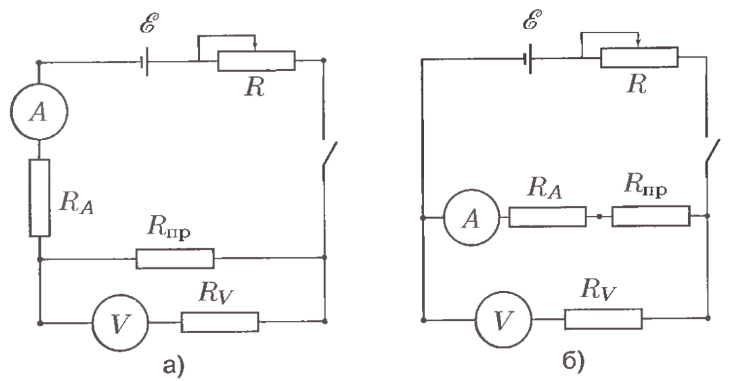
\includegraphics[width=11cm]{1}}
\end{center}

На данных схемах $R_V$ и $R_A$ -- сопротивления вольтметра и амперметра соответственно, а $R$ -- сопротивление реостата.

Для схемы a) имеем:
\[R_{\text{пр1}} = \frac{V_a}{I_a} = R_{\text{пр}} \frac{R_V}{R_V + R_{\text{пр}}} \]

Здесь $R_{\text{пр1}}$ -- измеренное сопротивление проволоки по закону Ома без учёта конечности сопротивления вольметра.

Для схемы б) имеем:
\[R_{\text{пр2}} = \frac{V_{\text{б}}}{I_{\text{б}}} = R_{\text{пр}} + R_A\]

Здесь $R_{\text{пр2}}$ -- измеренное сопротивление проволоки по закону Ома без учёта того, что у амперметра есть сопротивление.

Преобразуем оба выражения:
\[R_{\text{пр}} = R_{\text{пр1}} \frac{R_V}{R_V - R_{\text{пр1}}} = \frac{R_{\text{пр1}}}{1 - (R_{\text{пр1}})/(R_V)} \cong R_{\text{пр1}} (1 + \frac{R_{\text{пр1}}}{R_V})\]

\[R_{\text{пр}} = R_{\text{пр2}} (1 - \frac{R_A}{R_{\text{пр2}}})\]

Использовать надо то выражение, которое даёт меньшую поправку на сопротивление.\\

\section{Используемые оборудование и электрическая схема}

Так как известно, что $R_{\text{пр}}\cong 5$ Ом, оценим по ранее выведенным формулам поправки на сопротивление, учитывая, что $R_V = 10$ МОм и $R_A = 0,5$ Ом:

\[\frac{R_{\text{пр}}}{R_V} = 5 \cdot 10^{-6}, \text{ } \frac{R_A}{R_{\text{пр}}} = 1 \cdot 10^{-1} \Rightarrow \frac{R_{\text{пр}}}{R_V} \ll \frac{R_A}{R_{\text{пр}}}\]

Отсюда делаем вывод, что лучше использовать электрическую схему $a)$, так как она даёт значительно меньшую поправку на сопротивление проволоки.

\begin{center}
    \begin{tabular}{|c|c|}
        \hline
        Оборудование   & Погрешность измерения              \\
        \hline
        Штангенциркуль & 0,1 мм (маркировка производителя)  \\
        \hline
        Микрометр      & 0,01 мм (маркировка производителя) \\
        \hline
    \end{tabular}
\end{center}

\begin{center}
    \begin{tabular}{|c|c|c|}
        \hline
        \multicolumn{3}{|c|}{Характеристики амперметра и вольтметра} \\
        \hline
        Характеристики           & Вольтметр   & Амперметр           \\
        \hline
        Система                  & Цифровая    & Электромагнитная    \\
        \hline
        Цена деления             & 0,1 мВ      & 1 мА                \\
        \hline
        Число делений шкалы      & -           & 150                 \\
        \hline
        Чувствительность         & 10000 дел/В & 1000 дел/A          \\
        \hline
        Класс точности           & -           & 0,5                 \\
        \hline
        Предел измерений         & 5 В         & 150 мА              \\
        \hline
        Абсолютная погрешность   & 1мВ         & 0,75мА              \\
        \hline
        Внутреннее сопротивление & 10 МОм      & 0,3 Ом              \\
        \hline
    \end{tabular}
\end{center}
\newpage

\section{Результаты измерений диаметра проволоки}


Составим таблицу на основе измеренных данных толщины проволоки с помощью штангенциркуля и микрометра:

\begin{center}
    \begin{tabular}{|c|c|c|c|c|c|c|c|c|}
        \hline
                    & 1    & 2    & 3    & 4    & 5    & 6    & 7    & 8    \\
        \hline
        $d_{1},$ мм & 0,4  & 0,4  & 0,4  & 0,4  & 0,4  & 0,4  & 0,4  & 0,4  \\
        \hline
        $d_{2},$ мм & 0,36 & 0,36 & 0,36 & 0,37 & 0,35 & 0,36 & 0,36 & 0,35 \\
        \hline
    \end{tabular}
\end{center}

При измерении диаметра проволоки штангенциркулем случайная погрешность измерений отсутствует. Следовательно, точность результата определяется только точностью штангенциркуля (систематической погрешностью):
\[d_{1} = (0,4 \pm 0,1) \text{ мм}\]

Из полученных значений диаметров следует, что лучше пользоваться микрометром -- он более точный.

Посчитаем среднее значение для $d_{2}$: $\overline{d_{2}} = 0,358$ мм.

Для погрешностей имеем:
\[\sigma_{\text{сл}2} = \frac{1}{N}\sqrt{\sum_{i = 1}^{n}{(d_i-\overline{d_{0}})^2}} = 1,55\cdot 10^{-3} \text{ мм}\]
\[\sigma_{\text{сист}2} = 0,01 \text{ мм}\]

Поскольку $\sigma_{\text{сл}2}^2 \ll \sigma_{\text{сист}2}^2$, можно считать. что проволока однородна по диаметру и погрешность фактически определяется систематической:
\[d_{2} = \overline{d_{2}} \pm \sigma_d = (0,358 \pm 0,010) \text{ мм} =  (3,58 \pm 0,10)10^{-2} \text{ см}\]

Площадь поперечного сечения равна:
\[S = \frac{\pi \overline{d_{2}}^2}{4} = 1,01\cdot 10^{-3}\text{ см}^{2}\]

Погрешность определим через формулу погрешностей косвенных измерений:
\[\sigma_S = \frac{\partial{S}}{\partial{d}}\sigma_d = \frac{2S}{\overline{d_{2}}}\sigma_d = 5,6\cdot 10^{-5}\text{ см}^{2}\]\\\\\\


Итак, $S = (1,010 \pm 0,056)\cdot10^{-3} \text{ см}^{2}$

\section{Результаты измерений сопротивления проволоки}

Соберём электрческую схему $a)$ и проводим измерения вольт-амперной характеристики для трёх величин длины проволоки:\\ $l_1=(20\pm 0,1)$ см, $l_2=(30\pm 0,1)$ см, $l_3=(50\pm 0,1)$ см

Для большей точности измерения вольт-амперной характеристики проведём при возрастающих и убывающих значениях тока. Все показания приборов заносим в таблицу:

\begin{center}
    \begin{tabular}{|c|c|c|c|c|c|}
        \hline
        \multicolumn{6}{|c|}{Измерение напряжения и силы тока на проволоке}                                                                  \\ \hline
        \multicolumn{2}{|c|}{$L = 20$ см} & \multicolumn{2}{|c|}{$L = 30$ см} & \multicolumn{2}{|c|}{$L = 50$ см}                            \\ \hline
        $U$, В                            & $I$, А                            & $U$, В                            & $I$, А & $U$, В & $I$, А \\ \hline
        0,089                             & 0,031                             & 0,107                             & 0,032  & 0,168  & 0,031  \\ \hline
        0,100                             & 0,046                             & 0,150                             & 0,045  & 0,248  & 0,045  \\ \hline
        0,135                             & 0,062                             & 0,200                             & 0,060  & 0,330  & 0,060  \\ \hline
        0,166                             & 0,077                             & 0,250                             & 0,075  & 0,409  & 0,075  \\ \hline
        0,195                             & 0,091                             & 0,298                             & 0,090  & 0,496  & 0,091  \\ \hline
        0,227                             & 0,105                             & 0,347                             & 0,105  & 0,575  & 0,105  \\ \hline
        0,260                             & 0,122                             & 0,398                             & 0,120  & 0,664  & 0,122  \\ \hline
        0,289                             & 0,135                             & 0,447                             & 0,135  & 0,736  & 0,135  \\ \hline\hline
        0,265                             & 0,123                             & 0,398                             & 0,120  & 0,658  & 0,121  \\ \hline
        0,229                             & 0,106                             & 0,351                             & 0,106  & 0,568  & 0,104  \\ \hline
        0,194                             & 0,090                             & 0,296                             & 0,090  & 0,497  & 0,091  \\ \hline
        0,164                             & 0,076                             & 0,248                             & 0,075  & 0,413  & 0,075  \\ \hline
        0,131                             & 0,060                             & 0,198                             & 0,060  & 0,331  & 0,061  \\ \hline
    \end{tabular}
\end{center}

Строим графики зависимостей $U(I)$ для всех трёх длин отрезков проволки, проводя прямые через экспериментальные точки.
Из графиков видно, что нет различия между значениями, полученными при возрастании и при уменьшении тока.

\begin{center}
    {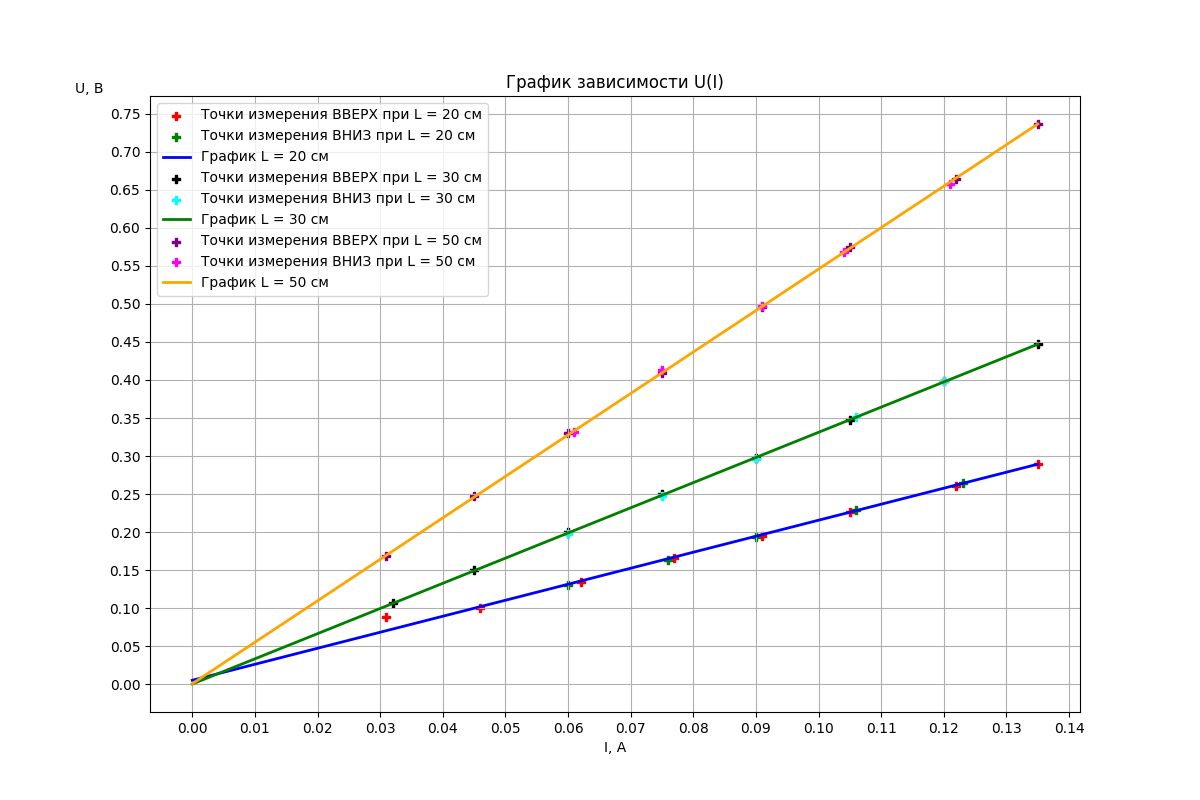
\includegraphics[width=22cm, height=13cm, angle=90]{2}}
\end{center}

Далее снимаем данные сопротивлений проволки при разных длинах с помощью моста Уитстона, записываем в таблицу.

Пользуясь методом наименьших квадратов, строим аппроксимирующие прямые $U_{B} = R_{\text{ср}}I_{A}$, определяя их угловой коэффициент по формуле


\[R_{\text{ср}} = \frac{\langle UI \rangle}{\langle I^2 \rangle}\]


Случайную погрешность определения углового коэффициента вычисляем как
\[\sigma_{R_{\text{ср}}}^{\text{случ}} = \frac{1}{\sqrt{n}}\sqrt{\frac{\langle U^2 \rangle}{\langle I^2 \rangle}- R_{\text{ср}}^2}.\]


(где n = 13 – число точек на графике).


Оценим возможную систематическую погрешность, обусловленную инструментальными
погрешностями приборов. Предполагая, что при всех измерениях относительная погрешность приборов одинакова, оценим погрешность вычисления частного R = U/I при максимальных
значениях U и I:
\[\sigma_{R_\text{ср}}^{\text{сист}} = R_\text{ср} \sqrt{\left(\frac{\sigma{_{U}}}{U_{max}}\right)^2 + \left( \frac{\sigma{_{I}}}{I_{max}}\right)^2}\]

$\sigma_V$ и $\sigma_I$ - ошибки измерения вольметром и амперметром. Они равны половине соответстующих абсолютных погрешностей приборов.

\[\sigma_V = \frac{1\text{ мВ}}{2} = 0,5 \text{ мВ} \]
\[\sigma_I = \frac{0,75\text{ мА}}{2} \sim 0,4 \text{ мА} \]


Складываем случайную и системптическую ошибки по формуле
\[\sigma_R = \sqrt{(\sigma_{R_{\text{ср}}}^{\text{случ}})^2 + (\sigma_{R_\text{ср}}^{\text{сист}})^2}\]


Внесём поправку в значения сопротивлений с помощью формулы:

\[R_{\text{пр}} = R_{\text{ср}} (1 + \frac{R_{\text{ср}}}{R_V})\]

Так как попроавка очень мала, можно считать, что $\sigma_{R_{\text{пр}}} = \sigma_{R_{\text{полн}}}$.

Результаты расчётов и измерений сведем в таблицу:

\begin{center}
    \begin{tabular}{|c|c|c|c|}
        \hline
        $L$, см                                    & 20      & 30      & 50      \\
        \hline
        \hline
        $R_{0}$, Ом                                & $2,182$ & $3,322$ & $5,449$ \\
        \hline
        $R_{\text{ср}}$, Ом                        & $2,158$ & $3,312$ & $5,457$ \\
        \hline
        $R_{\text{пр}}$, Ом                        & $2,158$ & $3,312$ & $5,457$ \\
        \hline
        $\sigma_{R_{\text{ср}}}^{\text{случ}}$, Ом & $0,019$ & $0,003$ & $0,005$ \\
        \hline
        $\sigma_{R_\text{ср}}^{\text{сист}}$, Ом   & $0,008$ & $0,011$ & $0,017$ \\
        \hline
        $\sigma_{R}$, Ом                           & $0,020$ & $0,011$ & $0,018$ \\
        \hline
    \end{tabular}
\end{center}

Видно, что случайная составляющая измерения сопротивления мала,
а основной вклад вносят систематические приборные погрешности.
Контрольные измерения с помощью моста в пределах погрешности совпадают, за исключением измерений для 20 см.
Скорее всего это вызвано ошибками при проведении измерений.

\section{Вычисление удельного сопротивления}

Удельное сопротивление проволоки и его погрешность определяются формулами:
\[\rho = \frac{R_{\text{пр}}}{L} \frac{\pi \overline{d_{2}}^2}{4}, \text{ } \sigma_{\rho} = \rho \sqrt{\Big( \frac{\sigma_{R_{\text{пр}}}}{R_{\text{пр}}}\Big) ^2 + \Big(\frac{\sigma_S}{S} \Big)^2 + \Big(\frac{\sigma_L}{L} \Big)^2}\]

Здесь $\sigma_{L} = 0,1$ см.
Занесём все результаты в таблицу:
\begin{center}
    \begin{tabular}{|c|c|c|c|}
        \hline
        $L$, см                                   & 20     & 30     & 50     \\
        \hline
        $\rho \cdot 10^{-4}$, Ом$\cdot$см         & $1,09$ & $1,11$ & $1,10$ \\
        \hline
        $\sigma_{\rho}\cdot 10^{-6}$, Ом$\cdot$см & $6$    & $6$    & $6$    \\
        \hline
    \end{tabular}
\end{center}

Окончательно: $\rho = (1,10 \pm 0,06) \cdot 10^{-4} \text{ Ом} \cdot \text{см}$

\section{Обсуждение результатов и выводы}


В работе получено значение удельного сопротивления образца проволоки из нихромового сплава с точностью 5,5\%.
Табличные значения для нихрома лежат в диапазоне $\rho_{табл} = 0,97 .... 1,12\cdot10^{-4}$ Ом см в зависимости от состава.
Измеренные значения $\rho = (1,10 \pm 0,06) \cdot 10^{-4}$ Ом м попадают в этот диапазон в пределах двух стандартных отклонений.

\end{document}


\end{document}
